\documentclass{article}

% Language setting
% Replace `english' with e.g. `spanish' to change the document language
\usepackage[english]{babel}

% Set page size and margins
% Replace `letterpaper' with `a4paper' for UK/EU standard size
\usepackage[letterpaper,top=2cm,bottom=2cm,left=3cm,right=3cm,marginparwidth=1.75cm]{geometry}

% Useful packages
\usepackage{amsmath}
\usepackage{graphicx}
\usepackage[colorlinks=true, allcolors=blue]{hyperref}
\usepackage{listings}


\title{Resurrecting Dead Images}
\author{Pierre Misse-Chanabier}

\begin{document}
\maketitle

\begin{abstract}
Using images to develop software has proven very useful.
However an image may break for multiple reasons and not being able to open anymore.
For example when using a breakpoint in a method used by the system may prevent it to open.
We explain here how we were able to recover such an image.
\end{abstract}

\section{Introduction}

Have you ever had a Pharo image that does not open anymore ?
Hours or even days of work lost forever because you forgot to save your code outside of the image ?
It happens to all Pharo developers at some point.
And we all hate the existing solutions when a lot of code is involved.

\paragraph{Epicea.} Epicea is pretty much the best option we have.
Quite frankly, it saved me multiple times.
It is awesome in a number of cases, because it allows us to reapply the latest changes on the current image.
One image may be dead, but we are able to reconstruct it !
However Epicea is not as great when you have to apply back multiple sessions, ones that you forgot, and particularly when it touches sensitive code such as the Compiler.

\section{Real World Case Description}

\subsection{The Murder}

In the RMOD team, we currently have a student that is working on having multiple OS windows, rather than only one (ref).
While working on this project, he was modifying very sensitive user interface code.
At some point, he added a breakpoint to explore a method, and saved his image to be sure he would be able to recover if something went wrong.
He then closed the image.
This image still had the breakpoint in the method.

\noindent Later, he tries to open the image.\newline
Nothing.\newline
The Pharo Launcher stays silent.\newline

\subsection{The Investigation}

We followed advice from a colleague.

"If you can run images on your laptop but not from Pharo Launcher, I suggest you open Pharo Launcher, select an image you know it can be opened, right-click on it and click on 'copy launch command'. 
You will get the command PL use to run the image. 
Then you could try it directly from a shell and see what happens. 
It is often the best way to understand what is wrong when an image does not open."


\begin{figure}[ht]
    \centering
    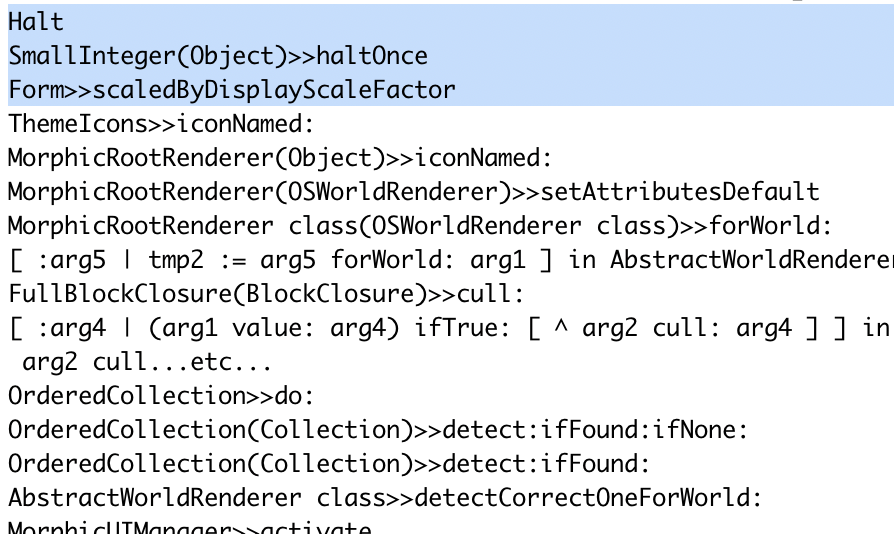
\includegraphics[width=0.7\linewidth]{debugStack}
    \caption{
    Debug stack printed by the VM when trying to open the image from a command line.
    This clearly shows that (1) the error preventing to open is indeed the halt and (2) the method containing the halt.
    }%
    \label{fig:debugStack}
\end{figure}

\noindent Following his advice, we found that the breakpoint is triggered by the startup of his image (Figure~\ref{fig:debugStack}).\newline
\noindent Therefore, the image cannot open the UI.\newline
\noindent Therefore, the image cannot open.\newline

\subsection{The Resurrection}

To fix this, we used a recent tool we wrote based on the VM simulator: \textbf{Polyphemus} \footnote{\url{https://github.com/hogoww/Polyphemus}}.
We opened the dead image inside a VM simulator, running inside a clean Pharo image.
We then explored the classes to find the class with the breakpoint method (Figure~\ref{fig:classBrowser}).

\begin{figure}[ht]
    \centering
    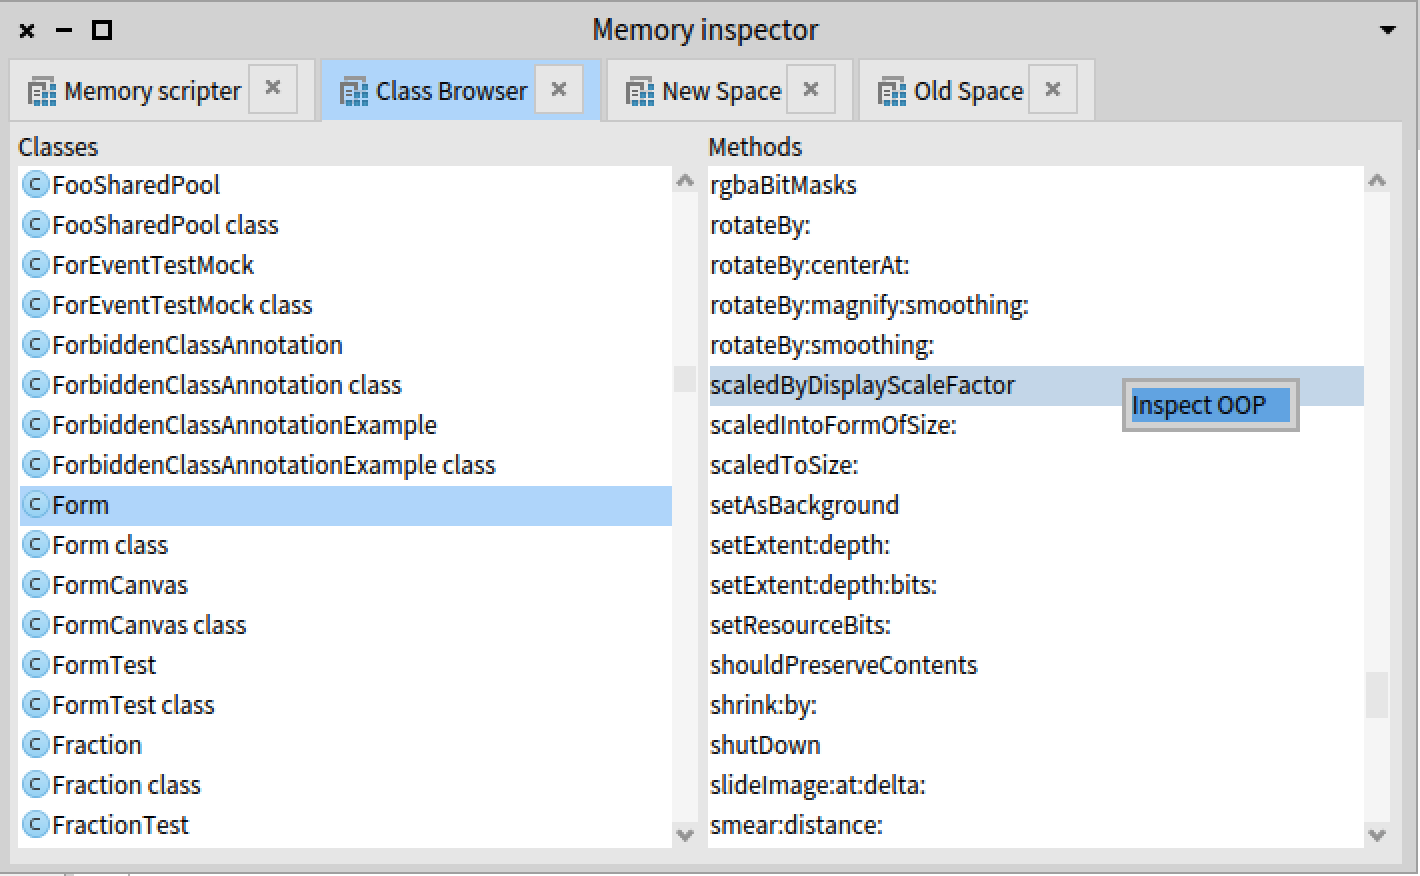
\includegraphics[width=0.9\linewidth]{classBrowser}
    \caption{Class browser.
    Allows to browse the classes and methods of the dead image.
    This allows to bypass the metacircularity of the environment and to browse the methods without executing any of them.
    }%
    \label{fig:classBrowser}
\end{figure}


\begin{figure}[ht]
    \centering
    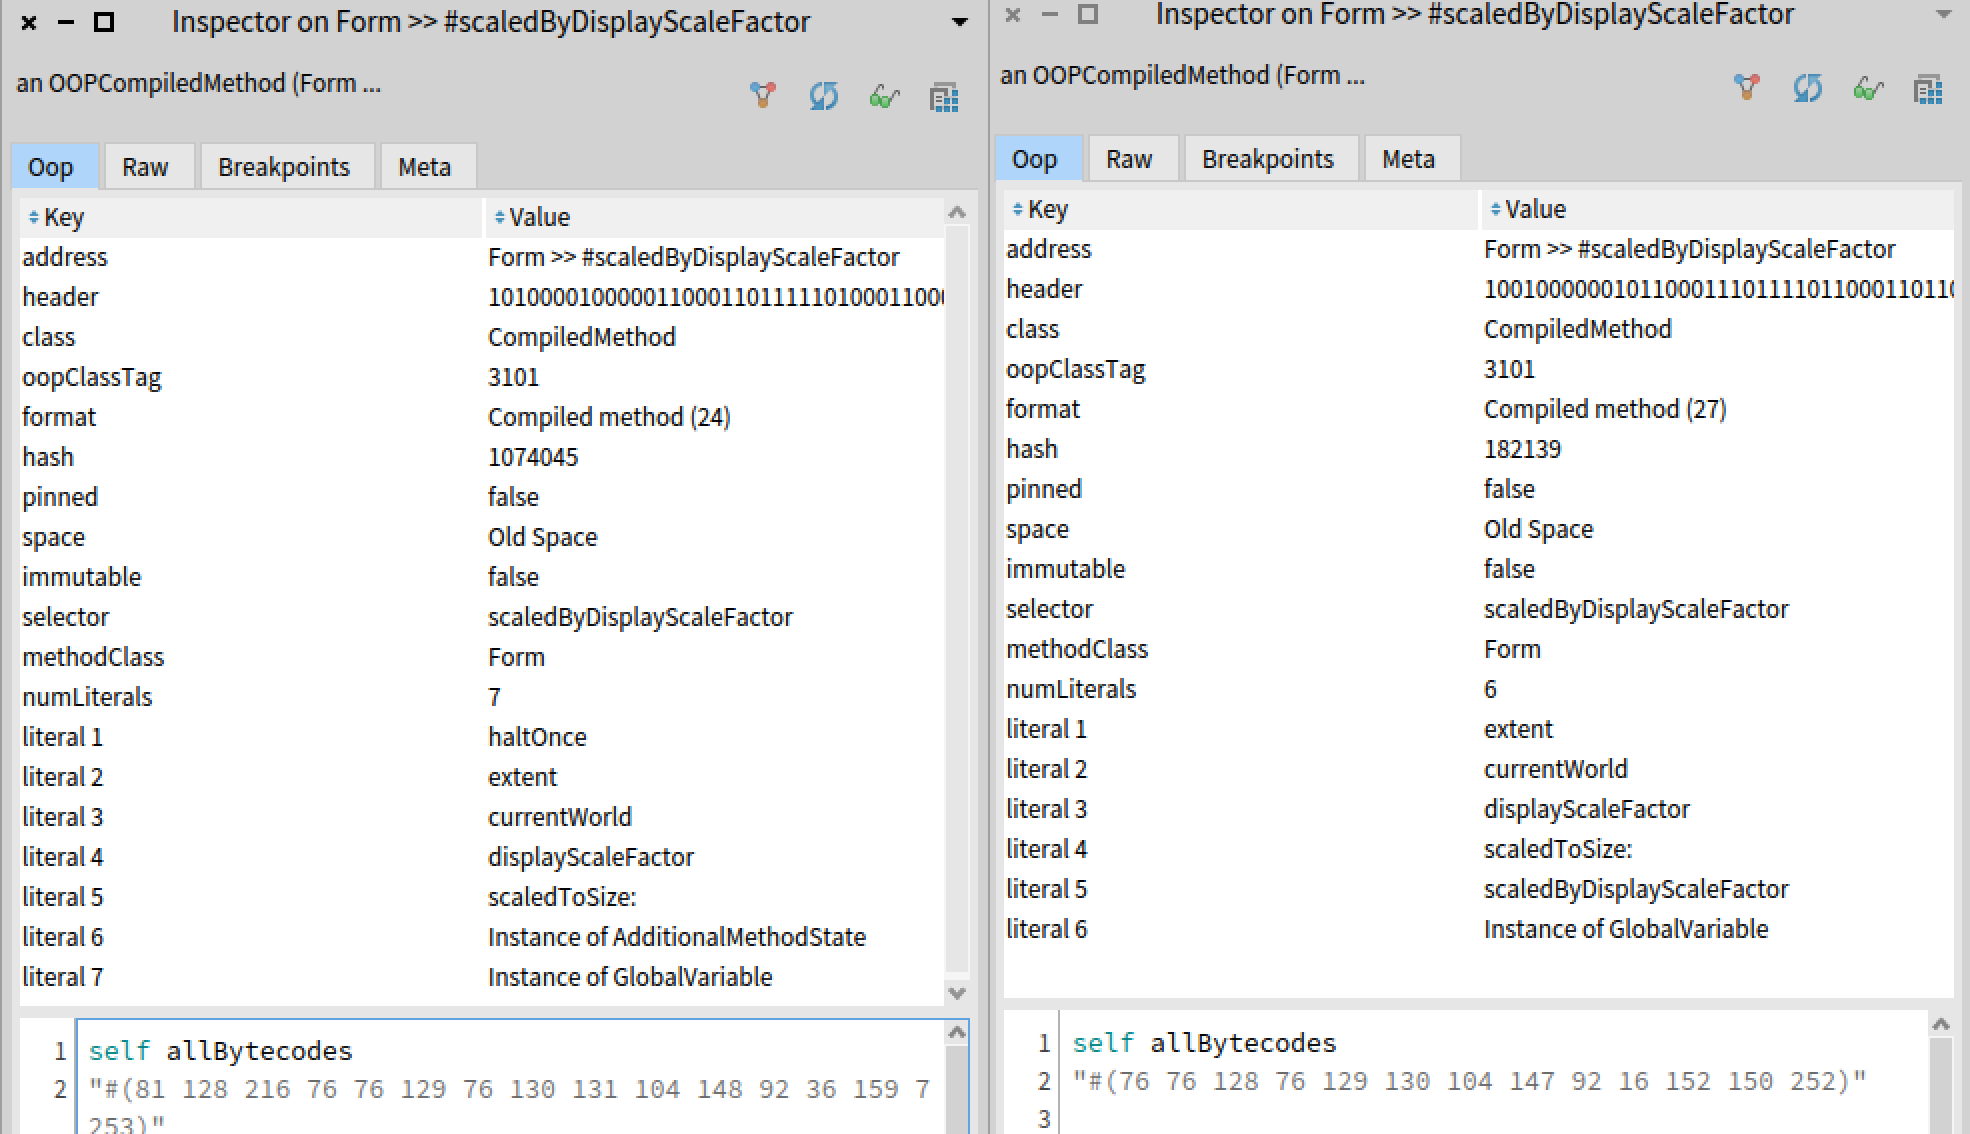
\includegraphics[width=0.9\linewidth]{methods}
    \caption{
    Inspection of the breakpoint compiled method object on the left and the clean compiled method object on the right.
    The breakpoint method has 3 more bytecodes sending the haltOnce message.
    It also has an extra literal for the selector \textit{\#haltOnce} in the first literal.
    }%
    \label{fig:methodObject}
\end{figure}

Once we had the method object (Figure~\ref{fig:methodObject}), we were able to compare the breakpoint version of this method, with one from a fresh Pharo 11, and analyse what we had to fix.

Of course, we first had to change the bytecodes.
We take the bytecode from the Pharo version and inject it into the image.
We replaced manually the content of this object with bytecodes that would execute the correct behavior.
We replaced the last extra bytecodes with 0.


\begin{lstlisting}[
    caption={Using Polyphemus to replace the bytecodes.
    \textbf{replacementsBytecodes} are the ones extracted from the correct method.
    We replaced the last few bytecodes with 0},
    label={lst:bytecodeFix}
    ]
    replacementBytecodes := #(76 76 128 76 129 130 104 147 92 16 152 150 252 0 0 0).
    replacementBytecodes doWithIndex: [ :aBytecode :anIndex |
        self bytecodeAt: anIndex put: aBytecode
    ]
\end{lstlisting}



\begin{lstlisting}[
    caption={Using Polyphemus to replace the literals.
    We replace each bytecode with the next one.},
    label={lst:literalFixes}
    ]
    0 to: self numberOfLiterals - 1 
        do: [ :aLiteralIndex | | nextLiteral |
            nextLiteral := self literalAt: aLiteralIndex + 1.
            self literalAt: aLiteralIndex put: nextLiteral
        ]
\end{lstlisting}



This also required fixing the method literals, which are used to express the breakpoint.
To send a message, the bytecode pushes the selector of that message on the execution stack.
To have this selector available, it is stored inside the method literals.
In this case, we can see that the \textit{haltOnce} selector is stored at index one (ref).
Therefore, the literals were off by one, and the indexes used by the bytecodes were wrong.
To fix that, we replace each literal by the next one.
This leaves a duplicated literal in the last index.
This is not really a problem, because it is not used in the bytecode.
This could be a problem because the last and penultimate literals have particular properties.
They hold the class and the selector of the method.
Therefore we advised the student to immediately recompile the method for safety !


\begin{lstlisting}[
    caption={Using the simulator to snapshot the memory onto the hard-drive.},
    label={lst:snapshots}
    ]
    reifiedMemory simulator coInterpreter primitiveSnapshot.
\end{lstlisting}

Finally, we snapshot this image~\ref{lst:snapshots}.
And poof, dead image is now resurrected !

With the abstractions provided by Polyphemus, it took us less than an hour to fix this image and recover days of work.

Note that this solution was possible because the method with the breakpoint has both more bytecodes and literals than the clean one.
Therefore we were able to keep it simple and just patch it.
More complex solutions would be required for more complex cases.


\section{Closing Words}

Although rudimentary, these solutions were achievable because of the initial effort of reifying the objects inside the VM simulator.
We are also investigating how to investigate and repair images suffering from memory corruption.
At this time, Polyphemus is just a base.
A base that took a lot of thinking and effort to create, but a base nonetheless.
The tools are yet to come !


\end{document}